\begin{activity} \label{A:9.2.5}

\begin{figure}[h]
  \begin{center}
    \begin{minipage}{3in}
      \begin{center}
        % \resizebox{!}{2.25in}{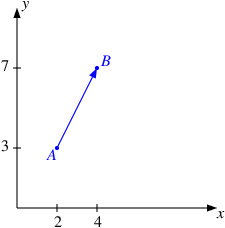
\includegraphics{figures/9_2_Vector_magnitude1}}
        \includegraphics{figures/fig-9-19-activity.eps}
      \end{center}
      \caption{} %$\overrightarrow{AB}$.
      \label{F:9.2.vector_activity1}
    \end{minipage}
    \begin{minipage}{3in}
      \begin{center}
        % \resizebox{!}{2.25in}{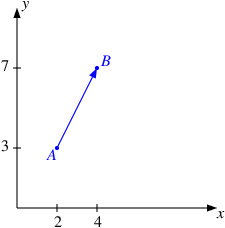
\includegraphics{figures/9_2_Vector_magnitude1}}
        \includegraphics{figures/fig-9-19-activity.eps}
      \end{center}
      \caption{} %$\overrightarrow{AB}$.
      \label{F:9.2.vector_activity2}
    \end{minipage}
  \end{center}
\end{figure}

Suppose that $\vu$ and $\vv$ are the vectors shown in Figure
\ref{F:9.2.vector_activity1}.   
	\ba
	\item On Figure \ref{F:9.2.vector_activity1}, sketch the
          vectors $\vu + \vv$, $\vv - \vu$, $2\vu$, $-2\vu$, and $-3\vv$. 
        \item What is $0\vv$?
        \item On Figure \ref{F:9.2.vector_activity2}, sketch the
          vectors $-3\vv$, $-2\vv$, $-1\vv$, $2\vv$, and $3\vv$.
        \item Give a geometric description of the set of vectors
          $t\vv$ where $t$ is any scalar.
        \item On Figure \ref{F:9.2.vector_activity2}, sketch the
          vectors $\vu-3\vv$, $\vu-2\vv$, $\vu-\vv$, $\vu + \vv$, and
          $\vu + 2\vv$.  
        \item Give a geometric description of the set of vectors
          $\vu + t\vv$ where $t$ is any scalar.

	\ea


\end{activity}
\begin{smallhint}

\end{smallhint}
\begin{bighint}

\end{bighint}
\begin{activitySolution}
	\ba
	\item A sketch of the vectors is shown below at left. 
    \item If we multiply any vector by the zero scalar, each component of the vector is multiplied by 0, resulting in the zero vector. So $0\vv = \vzero$.
    \item A sketch of the vectors is shown below at left. 
    \item This is the line through the origin in the direction of the vector $\vv$. 
     \item The vectors are shown below at right. 
\begin{center}
        \resizebox{!}{2.25in}{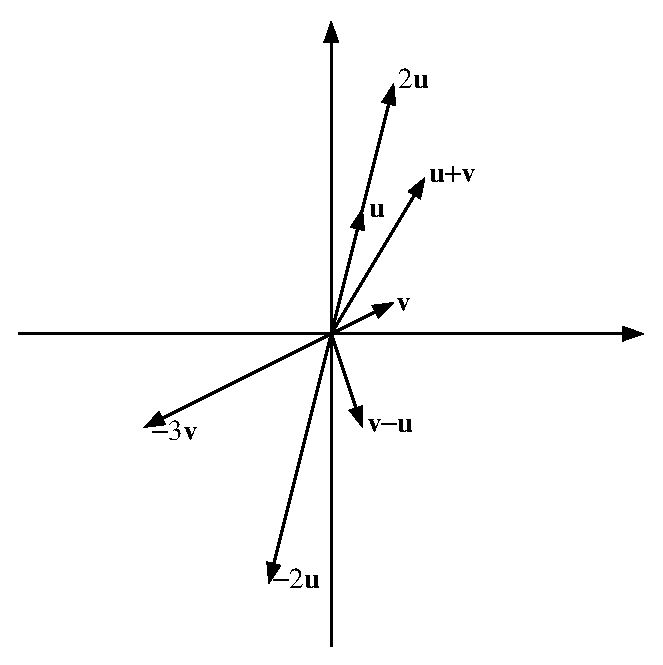
\includegraphics{figures/9_2_Act_5_Vectors_a}} \ \ \resizebox{!}{2.25in}{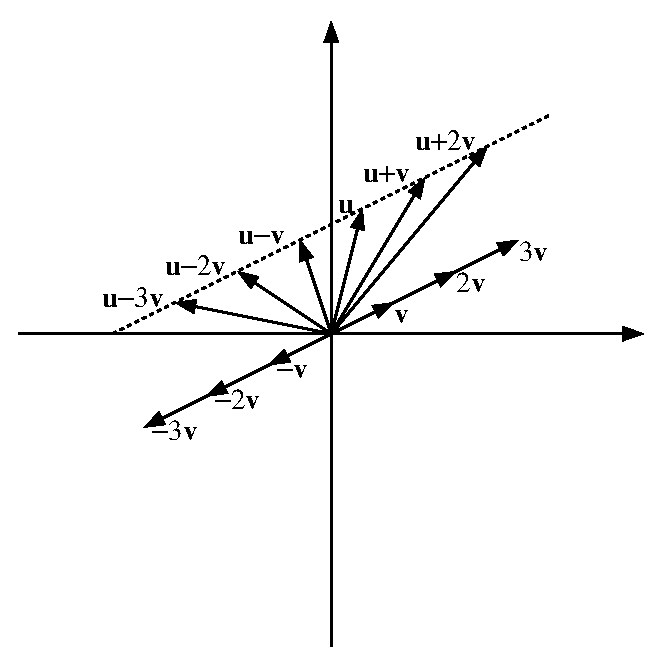
\includegraphics{figures/9_2_Act_5_Vectors_b}}
      \end{center}
     \item As the figure in part (e) illustrates, this is a line through the terminal point of the vector $\vu$ in standard position in the direction of the vector $\vv$. 
	\ea
\end{activitySolution}
\aftera
